\chapter{Proposed approach using Fully Convolutional Networks}\label{chap:proposed_model}

In this chapter the proposed models are described. These consist in FCN based deep learning architectures which are compared in the same datasets to ensure validated results and also to choose the best performing model for further analysis. The architectures are described using baseline parameters that will then be optimized using a grid search. In figure \ref{fig:flowchart} a flowchart of the proposed framework is shown.

\section{Segmentation architectures}
The architectures used are FCN based, so they share they building blocks shown in figure \ref{fig:fcn}. There is a contracting path of successive convolution and pooling layers and then an expanding path that mirrors the shape of the contracting one by applying transposed convolutions (upsampling) instead of pooling. Also, in the contracting path the number of feature maps increases while in the expanding path it decreases until reaching the output's number of channels. The segmentation architectures used are:

\begin{itemize}
    \item \textbf{DeconvNet:} This network is an FCN which uses a VGGNet \cite{vggnet} as a backbone for the contracting path. The expanding path mirrors the VGGNet architecture. Since it is based in a network that has already proven to have good results with image data it is appropriate to extend its application \cite{vggnet, Noh}. In figure \ref{fig:deconv} the contracting path is shown.

    \item \textbf{U-Net:} The U-Net is an FCN that was first implemented in the biomedical field for microscopy images. The architecture is shown in figure \ref{fig:unet} and makes use of skip layers which are taken from the contracting path and then concatenated in the expanding path layers. This allows the network to localize specific data by reducing dimensionality and also have the context of the general image through the skip layers \cite{Ronneberger}.
    


    \item \textbf{MultiResUnet:} This is an improvement of the U-Net, than can process subjects which have large differences in scale within an image. This is done with several convolutions with different kernels so that the features are learned at different resolutions, this is borrowed from Inception architectures such as GoogLeNet \cite{inception}. The structure is the same as in figure \ref{fig:unet} but the convolution blocks are changed with residual blocks that apply different convolutions which are then summed. Also, skip connections have a residual residual path in between. Figure \ref{fig:multires} shows the residual block used and figure \ref{fig:respath} depicts the residual connections used in the skip layers.
\end{itemize}

\begin{figure}
    \centering
     \resizebox{\linewidth}{!}{
    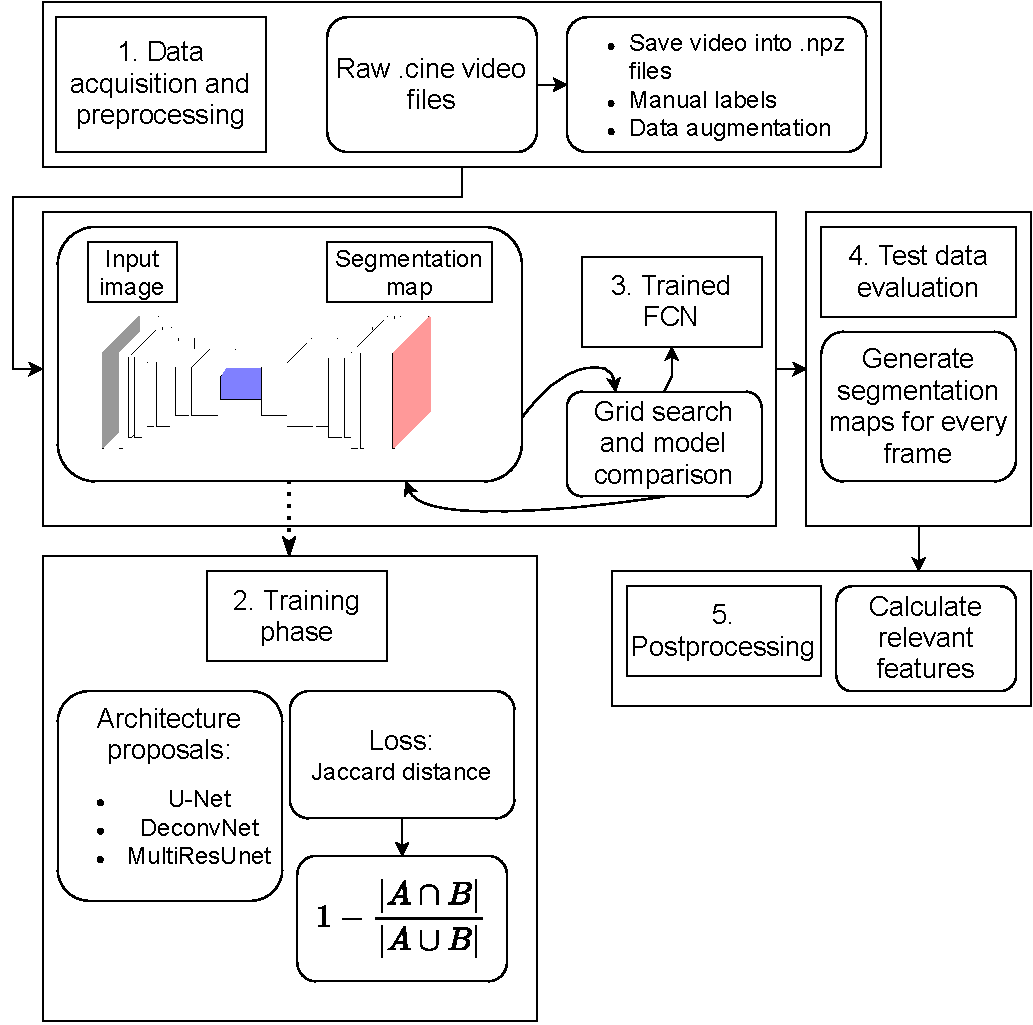
\includegraphics{Images/Background/framework_flow_chart.pdf}
    }
    \caption[Proposed framework flowchart]{Proposed framework flowchart.}
    \label{fig:flowchart}
\end{figure}

\begin{figure}
    \centering
    \resizebox{\linewidth}{!}{
    \begin{tikzpicture}
\tikzstyle{connection}=[ultra thick,every node/.style={sloped,allow upside down},draw=\edgecolor,opacity=0.7]
\tikzstyle{copyconnection}=[ultra thick,every node/.style={sloped,allow upside down},draw={rgb:blue,4;red,1;green,1;black,3},opacity=0.7]

%%%%%%%%%%%%%%%%%%%%%%%%%%%%%%%%%%%%%%%%%%%%%%%%%%%%%%%%%%%%%%%%%%%%%%%%%%%%%%%%%%%%%%%%
%% Draw Encoder
%%%%%%%%%%%%%%%%%%%%%%%%%%%%%%%%%%%%%%%%%%%%%%%%%%%%%%%%%%%%%%%%%%%%%%%%%%%%%%%%%%%%%%%%
% conv1_1,conv1_2
\pic[shift={(0,0,0)}] at (0,0,0) {RightBandedBox={name=cr1,%
        xlabel={{"64","64"}},zlabel=I,fill=\ConvColor,bandfill=\ConvReluColor,%
        height=40,width={2,2},depth=40}};
%pool1
\pic[shift={(0,0,0)}] at (cr1-east) {Box={name=p1,%
        fill=\PoolColor,opacity=0.5,height=32,width=1,depth=32}};
%%%%%%%%%%
% conv2_1,conv2_2
\pic[shift={(1,0,0)}] at (p1-east) {RightBandedBox={name=cr2,%
        xlabel={{"128","128"}},zlabel=I/2,fill=\ConvColor,bandfill=\ConvReluColor,%
        height=32,width={3.5,3.5},depth=32}};
%pool2
\pic[shift={(0,0,0)}] at (cr2-east) {Box={name=p2,%
        fill=\PoolColor,opacity=0.5,height=25,width=1,depth=25}};
%%%%%%%%%%
% conv3_1,conv3_2
\pic[shift={(0.75,0,0)}] at (p2-east) {RightBandedBox={name=cr3,%
        xlabel={{"256","256"}},zlabel=I/4,fill=\ConvColor,bandfill=\ConvReluColor,%
        height=25,width={4.5,4.5},depth=25}};
%pool3
\pic[shift={(0,0,0)}] at (cr3-east) {Box={name=p3,%
        fill=\PoolColor,opacity=0.5,height=16,width=1,depth=16}};
%%%%%%%%%%
% conv4_1,conv4_2,conv4_3
\pic[shift={(0.5,0,0)}] at (p3-east) {RightBandedBox={name=cr4,%
        xlabel={{"512","512"}},zlabel=I/8,fill=\ConvColor,bandfill=\ConvReluColor,%
        height=16,width={6,6},depth=16}};
%pool4
\pic[shift={(0,0,0)}] at (cr4-east) {Box={name=p4,%
        fill=\PoolColor,opacity=0.5,height=8,width=1,depth=8}};
%%%%%%%%%%%%%%%%%%%%%%%%%%%%%%%%%%%%%%%%%%%%%%%%%%%%%%%%%%%%%%%%%%%%%%%%%%%%%%%%%%%%%%%%
%% Bottleneck
%%%%%%%%%%%%%%%%%%%%%%%%%%%%%%%%%%%%%%%%%%%%%%%%%%%%%%%%%%%%%%%%%%%%%%%%%%%%%%%%%%%%%%%%% conv5_1,conv5_2,conv5_3
\pic[shift={(0.75,0,0)}] at (p4-east) {RightBandedBox={name=cr5,%
        xlabel={{"1024","1024"}},zlabel=I/16,fill=\ConvColor,bandfill=\ConvReluColor,%
        height=8,width={8,8},depth=8}};
%%%%%%%%%%%%%%%%%%%%%%%%%%%%%%%%%%%%%%%%%%%%%%%%%%%%%%%%%%%%%%%%%%%%%%%%%%%%%%%%%%%%%%%%
%% Draw Decoder 
%%%%%%%%%%%%%%%%%%%%%%%%%%%%%%%%%%%%%%%%%%%%%%%%%%%%%%%%%%%%%%%%%%%%%%%%%%%%%%%%%%%%%%%%
%% unpool4, 
\pic[shift={(1.2,0,0)}] at (cr5-east) {Box={name=up4,%
        fill=\UnpoolColor,opacity=0.6,height=16,width=1,depth=16}};
\pic[shift={(0,0,0)}] at (up4-east) {RightBandedBox={name=ucr4,%
        xlabel={{"512","dummy"}},fill=\ConvColor,bandfill=\ConvReluColor,%
        height=16,width=6,depth=16}};
\pic[shift={(0,0,0)}] at (ucr4-east) {RightBandedBox={name=cat4,%
        xlabel={{"512",""}},fill={rgb:white,1;black,3},bandfill={rgb:white,1;black,2},opacity=0.2,height=16,width=6,depth=16}};    
\pic[shift={(0,0,0)}] at (cat4-east) {RightBandedBox={name=ucr4a,%
        xlabel={{"512","512"}},zlabel=I/8,fill=\ConvColor,bandfill=\ConvReluColor,%
        height=16,width={6,6},depth=16}};
%%%%%%%%%%
%% unpool3, 
\pic[shift={(1.5,0,0)}] at (ucr4a-east) {Box={name=up3,%
        fill=\UnpoolColor,opacity=0.6,height=25,width=1,depth=25}};
\pic[shift={(0,0,0)}] at (up3-east) {RightBandedBox={name=ucr3,%
        xlabel={{"256","dummy"}},fill=\ConvColor,bandfill=\ConvReluColor,%
        height=25,width=4.5,depth=25}};
\pic[shift={(0,0,0)}] at (ucr3-east) {RightBandedBox={name=cat3,%
        xlabel={{"256",""}},fill={rgb:white,1;black,3},bandfill={rgb:white,1;black,2},opacity=0.2,height=25,width=4.5,depth=25}};
\pic[shift={(0,0,0)}] at (cat3-east) {RightBandedBox={name=ucr3a,%
        xlabel={{"256","256"}},zlabel=I/4,fill=\ConvColor,bandfill=\ConvReluColor,%
        height=25,width={4.5,4.5},depth=25}};
%%%%%%%%%%
%% unpool2, 
\pic[shift={(1,0,0)}] at (ucr3a-east) {Box={name=up2,%
        fill=\UnpoolColor,opacity=0.6,height=32,width=1,depth=32}};
\pic[shift={(0,0,0)}] at (up2-east) {RightBandedBox={name=ucr2,%
        xlabel={{"128","dummy"}},fill=\ConvColor,bandfill=\ConvReluColor,%
        height=32,width=3.5,depth=32}};
\pic[shift={(0,0,0)}] at (ucr2-east) {RightBandedBox={name=cat2,%
        xlabel={{"128",""}},fill={rgb:white,1;black,3},bandfill={rgb:white,1;black,2},opacity=0.2,height=32,width=3.5,depth=32}};    
\pic[shift={(0,0,0)}] at (cat2-east) {RightBandedBox={name=ucr2a,%
        xlabel={{"128","128"}},zlabel=I/2,fill=\ConvColor,bandfill=\ConvReluColor,%
        height=32,width={3.5,3.5},depth=32}};
%%%%%%%%%%
%% unpool1, 
\pic[shift={(1.5,0,0)}] at (ucr2a-east) {Box={name=up1,%
        fill=\UnpoolColor,opacity=0.6,height=40,width=1,depth=40}};
\pic[shift={(0,0,0)}] at (up1-east) {RightBandedBox={name=ucr1,%
        xlabel={{"64","dummy"}},fill=\ConvColor,bandfill=\ConvReluColor,%
        height=40,width=2.5,depth=40}};
\pic[shift={(0,0,0)}] at (ucr1-east) {RightBandedBox={name=cat1,%
        xlabel={{"64",""}},fill={rgb:white,1;black,3},bandfill={rgb:white,1;black,2},opacity=0.2,height=40,width=2.5,depth=40}};  
\pic[shift={(0,0,0)}] at (cat1-east) {RightBandedBox={name=ucr1a,%
        xlabel={{"64","64"}},fill=\ConvColor,bandfill=\ConvReluColor,%
        height=40,width={2.5,2.5},depth=40}};
%%%%%%%%%%%%%%%%%%%%%%%%%%%%%%%%%%%%%%%%%%%%%%%%%%%%%%%%%%%%%%%%%%%%%%%%%%%%%%%%%%%%%%%%
%% Classifier 
%%%%%%%%%%%%%%%%%%%%%%%%%%%%%%%%%%%%%%%%%%%%%%%%%%%%%%%%%%%%%%%%%%%%%%%%%%%%%%%%%%%%%%%%%
\pic[shift={(0.75,0,0)}] at (ucr1a-east) {Box={name=out,%
        zlabel=I,fill=\SoftmaxColor,height=40,width=1,depth=40}};
%%%%%%%%%%%%%%%%%%%%%%%%%%%%%%%%%%%%%%%%%%%%%%%%%%%%%%%%%%%%%%%%%%%%%%%%%%%%%%%%%%%%%%%
% Draw connections
%%%%%%%%%%%%%%%%%%%%%%%%%%%%%%%%%%%%%%%%%%%%%%%%%%%%%%%%%%%%%%%%%%%%%%%%%%%%%%%%%%%%%%%
\draw [connection]  (p1-east)    -- node {\midarrow} (cr2-west);
\draw [connection]  (p2-east)    -- node {\midarrow} (cr3-west);
\draw [connection]  (p3-east)    -- node {\midarrow} (cr4-west);
\draw [connection]  (p4-east)    -- node {\midarrow} (cr5-west);
\draw [connection]  (cr5-east)   -- node {\midarrow} (up4-west);
\draw [connection]  (ucr4a-east) -- node {\midarrow} (up3-west);
\draw [connection]  (ucr3a-east) -- node {\midarrow} (up2-west);
\draw [connection]  (ucr2a-east) -- node {\midarrow} (up1-west);
\draw [connection]  (ucr1a-east) -- node {\midarrow} (out-west);
%\draw [connection]  (out-east)   -- node {\midarrow} ++(2,0,0);

\path (cr4-southeast) -- (cr4-northeast) coordinate[pos=1.25] (cr4-top) ;
\path (cr3-southeast) -- (cr3-northeast) coordinate[pos=1.25] (cr3-top) ;
\path (cr2-southeast) -- (cr2-northeast) coordinate[pos=1.25] (cr2-top) ;
\path (cr1-southeast) -- (cr1-northeast) coordinate[pos=1.25] (cr1-top) ;

\path (cat4-south)  -- (cat4-north)  coordinate[pos=1.25] (cat4-top) ;
\path (cat3-south)  -- (cat3-north)  coordinate[pos=1.25] (cat3-top) ;
\path (cat2-south)  -- (cat2-north)  coordinate[pos=1.25] (cat2-top)  ;
\path (cat1-south)  -- (cat1-north)  coordinate[pos=1.25] (cat1-top)  ;
%
\draw [copyconnection]  (cr4-northeast)  
-- node {\copymidarrow}(cr4-top)
-- node {\copymidarrow}(cat4-top)
-- node {\copymidarrow} (cat4-north);
%
\draw [copyconnection]  (cr3-northeast)  
-- node {\copymidarrow}(cr3-top)
-- node {\copymidarrow}(cat3-top)
-- node {\copymidarrow} (cat3-north);
%
\draw [copyconnection]  (cr2-northeast)  
-- node {\copymidarrow}(cr2-top)
-- node {\copymidarrow}(cat2-top)
-- node {\copymidarrow} (cat2-north);
%
\draw [copyconnection]  (cr1-northeast)  
-- node {\copymidarrow}(cr1-top)
-- node {\copymidarrow}(cat1-top)
-- node {\copymidarrow} (cat1-north);

%%%%%%%%%%%%%%%%%%%%%%%%%%%%%%%%%%%%%%%%%%%%%%%%%%%%%%%%%%%%%%%%%%%%%%%%%%%%%%%%%%%%%%%
\end{tikzpicture}
    }
    \caption[Illustration of a U-Net architecture]{Illustration of a U-Net architecture. The architecture is divided in a contracting path and an expanding path. The contracting path has conv (yellow)/conv/pool (red) blocks. The expanding path has transposed-conv (blue)/conv/conv blocks. Dimensions in the expanding path mirror the contracting path. Each convolution before pooling is used as a skip layer and concatenated with the corresponding shape in the expanding path. The final layer reduces the feature maps to one and applies a softmax function for pixel-wise classification. Convolution kernels are $3\times 3$ while pooling kernels are $2\times 2$ so the size is halved at each block. Source: Adapted from \url{https://github.com/HarisIqbal88/PlotNeuralNet}.}
    \label{fig:unet}
\end{figure}

\begin{figure}
    \centering
    \resizebox{\linewidth}{!}{
    \begin{tikzpicture}
\tikzstyle{connection}=[ultra thick,every node/.style={sloped,allow upside down},draw=\edgecolor,opacity=0.7]
\tikzstyle{copyconnection}=[ultra thick,every node/.style={sloped,allow upside down},draw={rgb:blue,4;red,1;green,1;black,3},opacity=0.7]

%%%%%%%%%%%%%%%%%%%%%%%%%%%%%%%%%%%%%%%%%%%%%%%%%%%%%%%%%%%%%%%%%%%%%%%%%%%%%%%%%%%%%%%%
%% Draw Encoder
%%%%%%%%%%%%%%%%%%%%%%%%%%%%%%%%%%%%%%%%%%%%%%%%%%%%%%%%%%%%%%%%%%%%%%%%%%%%%%%%%%%%%%%%
% conv1_1,conv1_2
\pic[shift={(0,0,0)}] at (0,0,0) {RightBandedBox={name=cr1,%
        xlabel={{"64","64"}},ylabel=$3\times3$,zlabel=I,fill=\ConvColor,bandfill=\ConvReluColor,%
        height=40,width={2,2},depth=40}};
%pool1
\pic[shift={(0,0,0)}] at (cr1-east) {Box={name=p1,%
        fill=\PoolColor,opacity=0.5,height=32,width=1,depth=32,ylabel=$2\times2$}};
%%%%%%%%%%
% conv2_1,conv2_2
\pic[shift={(1,0,0)}] at (p1-east) {RightBandedBox={name=cr2,%
        xlabel={{"128","128"}},ylabel=$3\times3$,zlabel=I/2,fill=\ConvColor,bandfill=\ConvReluColor,%
        height=32,width={3.5,3.5},depth=32}};
%pool2
\pic[shift={(0,0,0)}] at (cr2-east) {Box={name=p2,%
        fill=\PoolColor,opacity=0.5,height=25,width=1,depth=25,ylabel=$2\times2$}};
%%%%%%%%%%
% conv3_1,conv3_2
\pic[shift={(0.75,0,0)}] at (p2-east) {RightBandedBox={name=cr3,%
        xlabel={{"256","256","256"}},ylabel=$3\times3$,zlabel=I/4,fill=\ConvColor,bandfill=\ConvReluColor,%
        height=25,width={4.5,4.5,4.5},depth=25}};
%pool3
\pic[shift={(0,0,0)}] at (cr3-east) {Box={name=p3,%
        fill=\PoolColor,opacity=0.5,height=16,width=1,depth=16,ylabel=$2\times2$}};
%%%%%%%%%%
% conv4_1,conv4_2,conv4_3
\pic[shift={(0.5,0,0)}] at (p3-east) {RightBandedBox={name=cr4,%
        xlabel={{"512","512","512"}},ylabel=$3\times3$,zlabel=I/8,fill=\ConvColor,bandfill=\ConvReluColor,%
        height=16,width={6,6,6},depth=16}};
%pool4
\pic[shift={(0,0,0)}] at (cr4-east) {Box={name=p4,%
        fill=\PoolColor,opacity=0.5,height=8,width=1,depth=8,ylabel=$2\times2$}};
%%%%%%%%%%%%%%%%%%%%%%%%%%%%%%%%%%%%%%%%%%%%%%%%%%%%%%%%%%%%%%%%%%%%%%%%%%%%%%%%%%%%%%%%
%% Bottleneck
%%%%%%%%%%%%%%%%%%%%%%%%%%%%%%%%%%%%%%%%%%%%%%%%%%%%%%%%%%%%%%%%%%%%%%%%%%%%%%%%%%%%%%%%% conv5_1,conv5_2,conv5_3
\pic[shift={(0.75,0,0)}] at (p4-east) {RightBandedBox={name=cr5,%
        xlabel={{"512","512","512"}},ylabel=$3\times3$,zlabel=I/16,fill=\ConvColor,bandfill=\ConvReluColor,%
        height=8,width={6,6,6},depth=8}};

%pool5
\pic[shift={(0,0,0)}] at (cr5-east) {Box={name=p5,%
        fill=\PoolColor,opacity=0.5,height=5,width=.7,depth=5,ylabel=$7\times7$}};
        
\pic[shift={(1,0,0)}] at (cr5-east) {RightBandedBox={name=fc,%
        xlabel={{"4096","4096"}},zlabel=I/32,fill=\ConvColor,bandfill=\ConvReluColor,%
        height=2,width={12,12},depth=2}};
%%%%%%%%%%%%%%%%%%%%%%%%%%%%%%%%%%%%%%%%%%%%%%%%%%%%%%%%%%%%%%%%%%%%%%%%%%%%%%%%%%%%%%%%
%% Draw Decoder 
%%%%%%%%%%%%%%%%%%%%%%%%%%%%%%%%%%%%%%%%%%%%%%%%%%%%%%%%%%%%%%%%%%%%%%%%%%%%%%%%%%%%%%%%

%%%%%%%%%%%%%%%%%%%%%%%%%%%%%%%%%%%%%%%%%%%%%%%%%%%%%%%%%%%%%%%%%%%%%%%%%%%%%%%%%%%%%%%
% Draw connections
%%%%%%%%%%%%%%%%%%%%%%%%%%%%%%%%%%%%%%%%%%%%%%%%%%%%%%%%%%%%%%%%%%%%%%%%%%%%%%%%%%%%%%%
\draw [connection]  (p1-east)    -- node {\midarrow} (cr2-west);
\draw [connection]  (p2-east)    -- node {\midarrow} (cr3-west);
\draw [connection]  (p3-east)    -- node {\midarrow} (cr4-west);
\draw [connection]  (p4-east)    -- node {\midarrow} (cr5-west);
\draw [connection]  (p5-east)    -- node {\midarrow} (fc-west);


%%%%%%%%%%%%%%%%%%%%%%%%%%%%%%%%%%%%%%%%%%%%%%%%%%%%%%%%%%%%%%%%%%%%%%%%%%%%%%%%%%%%%%%
\end{tikzpicture}
    }
    \caption[Illustration of a DeconvNet contracting path]{Illustration of a DeconvNet contracting path. A VGGNet architecture is used and then mirrored in the expanding path. At the top of each block the kernel shape is shown, below are depicted the number of feature maps per convolution. Finally, $I$ is the input size which is halved after each pooling layer. Source: Adapted from \url{https://github.com/HarisIqbal88/PlotNeuralNet}.}
    \label{fig:deconv}
\end{figure}
    
\begin{figure}
    \centering
    \resizebox{\linewidth}{!}{
    \begin{tikzpicture}
\tikzstyle{connection}=[ultra thick,every node/.style={sloped,allow upside down},draw=\edgecolor,opacity=0.7]
\tikzstyle{copyconnection}=[ultra thick,every node/.style={sloped,allow upside down},draw={rgb:blue,4;red,1;green,1;black,3},opacity=0.7]

%%%%%%%%%%%%%%%%%%%%%%%%%%%%%%%%%%%%%%%%%%%%%%%%%%%%%%%%%%%%%%%%%%%%%%%%%%%%%%%%%%%%%%%%
%% Draw Encoder
%%%%%%%%%%%%%%%%%%%%%%%%%%%%%%%%%%%%%%%%%%%%%%%%%%%%%%%%%%%%%%%%%%%%%%%%%%%%%%%%%%%%%%%%
% conv1_1,conv1_2
\def\ConvColor{rgb:red,50;green,227;blue,150}
\def\ConvReluColor{rgb:red,50;green,200;blue,100}

\pic[shift={(0,0,0)}] at (0,0,0) {RightBandedBox={name=cr1,ylabel=$3\times3$,fill=\ConvColor,bandfill=\ConvReluColor,%
        height=20,width={0.5},depth=20}};

\node[inner sep=0,minimum size=0] (o0) at (-2,0,0) {}; % invisible node

\node[inner sep=0,minimum size=0,right of=o0] (k0) {}; % invisible node

\node[inner sep=0,minimum size=0] (o1) at (0,0,0) {}; % invisible node

\node[inner sep=0,minimum size=0,right of=o1] (k1) {}; % invisible node

\node[inner sep=0,minimum size=0] (o2) at (2.3,0,0) {}; % invisible node

\node[inner sep=0,minimum size=0,right of=o2] (k2) {}; % invisible node

%%%%%%%%%%
% conv2_1,conv2_2
\pic[shift={(2,0,0)}] at (cr1-east) {RightBandedBox={name=cr2,%
        xlabel={{"",""}},ylabel=$3\times3$,fill=\ConvColor,bandfill=\ConvReluColor,%
        height=20,width={0.5,0.5},depth=20}};
%%%%%%%%%%
% conv3_1,conv3_2
\pic[shift={(2,0,0)}] at (cr2-east) {RightBandedBox={name=cr3,ylabel=$3\times3$,fill=\ConvColor,bandfill=\ConvReluColor,%
        height=20,width={0.5,0.5,0.5,0.5},depth=20}};

        
%%%%%%%%%%
% conv4_1,conv4_2,conv4_3
\pic[shift={(2,0,0)}] at (cr3-east) {RightBandedBox={name=cr4,ylabel=\hspace{-5pt}Concatenation,fill=\ConvColor,bandfill=\ConvReluColor,%
        height=10,width={3,3,3},depth=10}};

%%%%%%%%%%
% conv3_1,conv3_2
\pic[shift={(0,5,0)}] at (cr3-east) {RightBandedBox={name=id,ylabel=$1\times1$,fill=blue!20,bandfill=blue!20,%
        height=10,width={0.5},depth=10}};


\node[draw,circle,minimum size=1.6cm,inner sep=0pt, color = black, very thick, fill = black!5] (sum) at (12,0) {\Huge $\mathbf{+}$};

\node[inner sep=0,minimum size=0] (k3) at (15,0) {}; % invisible node
%%%%%%%%%%%%%%%%%%%%%%%%%%%%%%%%%%%%%%%%%%%%%%%%%%%%%%%%%%%%%%%%%%%%%%%%%%%%%%%%%%%%%%
% Draw connections
%%%%%%%%%%%%%%%%%%%%%%%%%%%%%%%%%%%%%%%%%%%%%%%%%%%%%%%%%%%%%%%%%%%%%%%%%%%%%%%%%%%%%%%
\draw node (I) at (-3,0,0) {Input};

\draw [connection]  (I)    -- node {\midarrow} (cr1-west);
\draw [connection]  (cr1-east)    -- node {\midarrow} (cr2-west);
\draw [connection]  (cr1-east)    -- node {\midarrow} (cr2-west);
\draw [connection]  (cr2-east)    -- node {\midarrow} (cr3-west);
\draw [connection]  (cr3-east)    -- node {\midarrow} (cr4-west);
\draw [connection]  (cr4-east)    -- node {\midarrow} (sum);
\draw [connection]  (sum)    -- node {\midarrow} (k3);



\draw [connection]  (k1) - ++(0,-4) -| node {\midarrow} (cr4-southeast);
\draw [connection]  (k2) - ++(0,-3) -| node {\midarrow} (cr4-south);
\draw [connection]  (k0) |- node {\midarrow} (id-west);
\draw [connection]  (id-east) -| node {\midarrow} (sum);




%%%%%%%%%%%%%%%%%%%%%%%%%%%%%%%%%%%%%%%%%%%%%%%%%%%%%%%%%%%%%%%%%%%%%%%%%%%%%%%%%%%%%%%
\end{tikzpicture}

    }
    \caption[Illustration of a Multi Resolution block]{Illustration of a Multi Resolution block. The block consists of successive convolutions which are then stacked via skip layers and then summed using a residual connection. The second and third convolutional blocks are stacked convolutions of $3\times3$ kernels which are factorized operations of $5\times 5$ and $7 \times7$ convolutions respectively \cite{conv-factor}. This approach is more computationally efficient than using parallel higher resolution kernels. Source: Adapted from \url{https://github.com/HarisIqbal88/PlotNeuralNet}.}
    \label{fig:multires}
\end{figure}

\begin{figure}
    \centering
    \resizebox{0.5\linewidth}{!}{
    \begin{tikzpicture}
\tikzstyle{connection}=[ultra thick,every node/.style={sloped,allow upside down},draw=\edgecolor,opacity=0.7]
\tikzstyle{copyconnection}=[ultra thick,every node/.style={sloped,allow upside down},draw={rgb:blue,4;red,1;green,1;black,3},opacity=0.7]

%%%%%%%%%%%%%%%%%%%%%%%%%%%%%%%%%%%%%%%%%%%%%%%%%%%%%%%%%%%%%%%%%%%%%%%%%%%%%%%%%%%%%%%%
%% Draw Encoder
%%%%%%%%%%%%%%%%%%%%%%%%%%%%%%%%%%%%%%%%%%%%%%%%%%%%%%%%%%%%%%%%%%%%%%%%%%%%%%%%%%%%%%%%
% conv1_1,conv1_2
\def\ConvColor{rgb:red,50;green,227;blue,150}
\def\ConvReluColor{rgb:red,50;green,200;blue,100}

\pic[shift={(0,0,0)}] at (0,0,0) {RightBandedBox={name=cr1,ylabel=$3\times3$,fill=\ConvColor,bandfill=\ConvReluColor,%
        height=15,width={0.5},depth=15}};

\node[inner sep=0,minimum size=0] (o0) at (-2,0,0) {}; % invisible node

\node[inner sep=0,minimum size=0,right of=o0] (k0) {}; % invisible node


%%%%%%%%%%
% conv3_1,conv3_2
\pic[shift={(2,4,0)}] at (cr1-east) {RightBandedBox={name=id,ylabel=$1\times1$,fill=blue!20,bandfill=blue!20,%
        height=10,width={0.5},depth=10}};


\node[draw,circle,minimum size=1cm,inner sep=0pt, color = black, very thick, fill = black!5] (sum) at (5,0) {\Huge $\mathbf{+}$};

\node[inner sep=0,minimum size=0] (k3) at (7,0) {}; % invisible node
%%%%%%%%%%%%%%%%%%%%%%%%%%%%%%%%%%%%%%%%%%%%%%%%%%%%%%%%%%%%%%%%%%%%%%%%%%%%%%%%%%%%%%
% Draw connections
%%%%%%%%%%%%%%%%%%%%%%%%%%%%%%%%%%%%%%%%%%%%%%%%%%%%%%%%%%%%%%%%%%%%%%%%%%%%%%%%%%%%%%%
\draw node (I) at (-3,0,0) {Input};

\draw [connection]  (I)    -- node {\midarrow} (cr1-west);
\draw [connection]  (cr1-east)    -- node {\midarrow} (sum);
\draw [connection]  (sum)    -- node {\midarrow} (k3);

\draw [connection]  (k0) |- node {\midarrow} (id-west);
\draw [connection]  (id-east) -| node {\midarrow} (sum);




%%%%%%%%%%%%%%%%%%%%%%%%%%%%%%%%%%%%%%%%%%%%%%%%%%%%%%%%%%%%%%%%%%%%%%%%%%%%%%%%%%%%%%%
\end{tikzpicture}
    }
    \caption[Illustration of a residual path]{Illustration of a residual path. This type of block is used in series in the MultiResUnet in between skip layers, so the skipped features are processed before being concatenated to the expanding path. Source: Adapted from \url{https://github.com/HarisIqbal88/PlotNeuralNet}.}
    \label{fig:respath}
\end{figure}

\clearpage
\section{Segmentation loss function}

As stated earlier, to train a supervised neural network it is necessary to have some measure of error so that it can be minimized with respect to the weights. This measure is the loss function which depends on the task. In the case of semantic segmentation, it is necessary to use a loss function that can capture pixel-wise comparisons. Specifically, for supervised segmentation, the input is an image, the output is a 2D mapping of each pixel of the image to a certain class (e.g. pixel$ = 0$ if background and pixel$ = 1$ if foreground) and the output is compared through the loss function with a previously labeled image with the same kind of segmentation mapping corresponding to the input image. A widely used loss metric for supervised semantic segmentation is the intersection over union metric, also known as Jaccard index. This metric is given by
\begin{align*}
    J(A, B) = \frac{|A\cap B|}{|A\cup B|}
\end{align*}
where $|\cdot|$ is the cardinality of the set. Hence, if the overlap is perfect $|A\cap B|=|A\cup B|\xrightarrow[]{} J=1$. Conversely, if there is no overlap $|A\cap B|=0\xrightarrow{} J=0$. In a segmentation mapping, $|A\cap B|$ can be computed as the element-wise multiplication of $A$ and $B$, and then sum the result. Furthermore, $|\cdot|$ is computed as the sum of the matrix' elements. The score is computed over all classes and then averaged.
    
In order to minimize a loss function using the Jaccard index, the Jaccard distance is used and is given by
\begin{align*}
    d_j(A,B)=1-J(A,B)
\end{align*}

\section{Validation}
The proposed architectures have to be validated to ensure that the best results are obtained. Then, every model is subject to a grid search. The parameters used for grid search are shown in table \ref{table:grid_search}. Also, each model (i.e. each point in the grid) is run using $k$-fold cross validation with $k=4$. That is, each model is run four times with a different and disjoint $25\%$ of validation data each time. The average loss in the validation set is used to compare the models' performances and choose the best one.

\begin{table}
\caption[Hyperparameters used for grid search]{Hyperparameters used for grid search.}
\label{table:grid_search}
\centering
\begin{tabular}{|c|c|c|c|c|}
\cline{1-2} \cline{4-5}
Dataset & (Globular, Spray) &  & \begin{tabular}[c]{@{}c@{}}Number \\ of filters\end{tabular} & (8, 16, 32) \\ \cline{1-2} \cline{4-5} 
Epochs & \begin{tabular}[c]{@{}c@{}}Early stopping\\ Max: 200 epochs\\ Patience: 20 epochs\end{tabular} &  & \begin{tabular}[c]{@{}c@{}}Learning\\ rate\end{tabular} & (.01, .005, .001) \\ \cline{1-2} \cline{4-5} 
\begin{tabular}[c]{@{}c@{}}Loss\\ function\end{tabular} & \begin{tabular}[c]{@{}c@{}}Jaccard\\ distance\end{tabular} &  & Optimizer & Adam \\ \cline{1-2} \cline{4-5} 
\begin{tabular}[c]{@{}c@{}}Batch\\ size\end{tabular} & (8, 16, 32) &  & Architecture & \begin{tabular}[c]{@{}c@{}}(U-Net, DeconvNet,\\ MultiResUnet)\end{tabular} \\ \cline{1-2} \cline{4-5} 
\end{tabular}
\end{table}

